\begin{savequote}[8cm]
  ``He who controls the past controls the future.''
  \qauthor{George Orwell, 1984}
\end{savequote}
\makeatletter
\chapter{Literature Review}

\section{Introduction}

3D model compression research has followed a path similar to image compression, with lossless codecs being proposed first, followed by lossy transform based methods. More recently though, novel hierarchical techniques have been developed. These techniques outperform transform and wavelet based approaches at low bit rates, and none of them have been extended to 3D. Research conducted in 3D model compression typically assumes the need to compress a particular representation rather than just compressing the 3D data. Therefore, it is necessary to survey the range of representation specific compression methods to understand the field.

\section{3D Data Representations}

\subsection{Introduction}

In order to understand 3D model codecs, it is imperative to present a background of popular 3D data representations. Each representation has certain advantages and disadvantages in terms of storage, transmission, processing, and visualization. Representations are divided into five unique categories: polygonal mesh, point cloud, volumetric, hierarchical \& depth image based.  The basic concept of each strategy is explained in each section, with special focus on hierarchical techniques.

\subsection{The Polygonal Mesh Representation}
\label{PolygonalMeshSection}
The polygon mesh representation has been the most popular representation for 3D data since the 1990s. This structure has been incorporated into graphics hardware technology and has thus received the majority of attention within the literature. This representation makes use of vertices, edges and polygons. For example, see the left image in figure \ref{MeshExamples}, vertices are represented as black dots, edges are represented by lines, and polygons are labelled $F_0, F_1, F_2, F_3, F_4$. Vertices represent geometric information whilst edges and polygons are forms of connectivity or topology information.

For ease of processing, polygonal models are often triangulated (all polygons are transformed into triangles). A majority of the polygon mesh processing algorithms require the object to be represented using triangles rather than polygons. Any polygonal mesh can be triangulated, an example of this is provided on the right hand side in figure \ref{MeshExamples}. Usually vertices are stored explicitly in a list, triangles are stored using three references to this vertex list and edges are stored implicitly. To measure storage requirements, two metrics often used are: bits per vertex (bpv) and bits per triangle (bpt). Peng \textit{et al.} \cite{Peng05Technologies} make the assumption that there are roughly twice as many triangles as there are vertices, this concept is used throughout this thesis to convert bpt to bpv.

%\begin{figure}[!h]
%\centering
%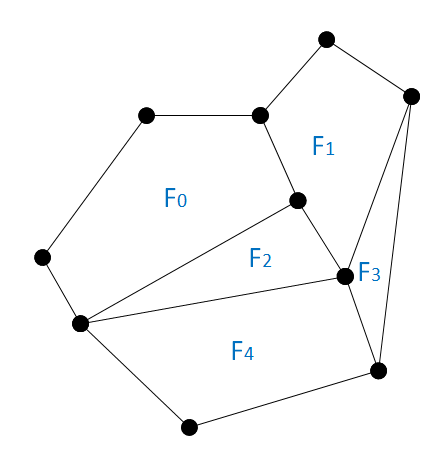
\includegraphics[width=6cm]{images/ch1/PolygonMeshExample}
%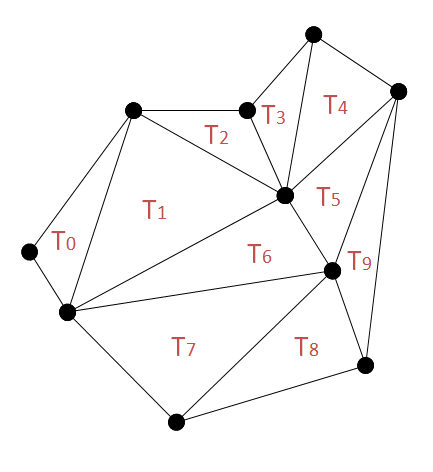
\includegraphics[width=6cm]{images/ch1/TriangleMeshExample}
%\caption{Left: Polygonal Mesh, Right: Triangulated Mesh}
%\label{MeshExamples}
%\end{figure}

Some mesh codecs place topological restrictions on the types of models they can compress. These restrictions are based on whether the mesh is manifold and/or orientable, both of these are summarized by Peng \textit{et al.} \cite{Peng05Technologies}. A 3D model is said to be manifold if it can be stretched and moulded into a sphere or a half sphere. An example of a manifold object is shown in figure \ref{ManifoldExample}, a manifold object is said to be homomorphic (of similar structure) to a disk. An object is orientable if each triangle shares an edge with at most one other triangle. 


%\begin{figure}[!t]
%\centering
%\includegraphics[width=12cm]{images/ch1/HomomorphicToADisk}
%\caption{A mesh progressively moulded into a disk, a mesh with this characteristic is said to be manifold.}
%\label{ManifoldExample}
%\end{figure}


\subsection{The Point Cloud Representation}

The point cloud structure stores only vertex information. This representation can be thought of as discrete samples of the surface of a 3D object. For a visual example of this data structure, see figure \ref{PointCloudExample}. This type of structure can be sampled using a variety of methods. These methods include both dense and sparse sampling, and sample steps can be either regular or irregular. Along with each vertex, a variety of attribute information can be stored. Point cloud data is usually obtained through the use of a 3D scanner. The point cloud has recently become popular in 3D compression research, although it is still not as frequently used as the mesh representation.

%\begin{figure}[!h]
%\centering
%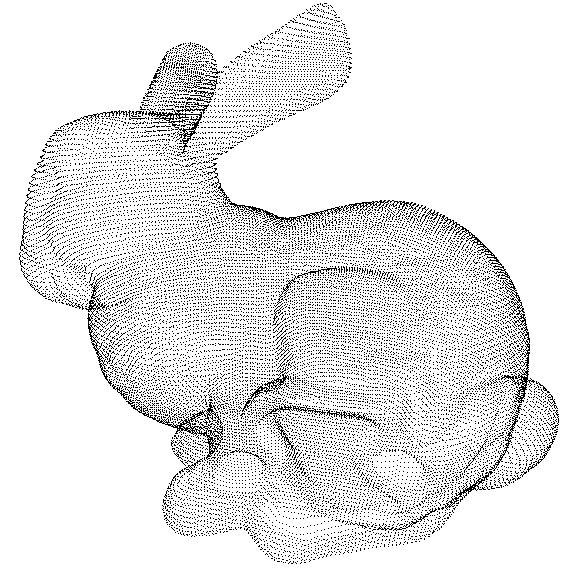
\includegraphics[width=6cm]{images/ch1/PointCloudExample}
%\caption{A densely sampled point cloud of the Stanford Bunny.}
%\label{PointCloudExample}
%\end{figure}

\subsection{The Volumetric Representation}

Volumetric data structures typically use a set of 3D primitives as building blocks for more complex 3D structures. Cubes are used most often because of their simplicity, but other primitives can also be used. Unlike the point cloud structure, the geometric data (the cubes) also contain volume information and are always regularly sampled. This structure can be thought of as a 3D image, with each cube (also called a voxel or volumetric pixel) corresponding to a pixel. An example of this structure is provided in figure \ref{VolumetricSurfaceExample}. It shows that when dense sampling is used, the visual quality approaches that of the original model. 

%\begin{figure}[!h]
%\centering
%\includegraphics[width=12cm]{images/ch1/VolumetricSurfaceExample}
%\caption{Left to right: Original Mesh, Sparsely Sampled Volumetric Model, Densely Sampled Volumetric Model.}
%\label{VolumetricSurfaceExample}
%\end{figure}



\subsection{Hierarchical Techniques}

Hierarchical techniques are used to represent 3D, audio and image data. When used to represent 3D objects the data can be transformed into a hierarchy from any other representation. Typical hierarchical structures used for 3D model representation include: the K-D tree, BSP-tree and the Octree (OT). Detailed information on these structures can be found in Hanan Samet's Foundations of Multidimensional and Metric Data Structures \cite{Samet06Foundations}. The OT and K-D tree have previously been used in 3D object compression, for both mesh \cite{Peng05Geometry-Guided} and surface data \cite{Schnabel06Octree}. Since the OT is a focus point for this thesis, it is described below.

\subsubsection{The Quadtree}

In order to understand the OT structure, the Quad-Tree (QT) is explained first. This is done because the QT is the 2D equivalent of the OT and is easier to explain. The QT is a hierarchical data structure used for processing and compressing 2D data. Figure \ref{QuadtreeExample} shows an example of a QT used to represent an image. In this figure, the original image is on the left. The QT first uses a single coloured square to represent the entire image, then using some error metric it decides whether or not to, a) represent the image more accurately using more memory or b) stop decomposition and represent the image with a single colour. If option b) is chosen, the image will look like the second left picture. If option a) is chosen, the image is divided into four sub-images each with its own colour. From here the whole process begins again, with each sub-image given the same options. The final product of the QT is shown on the far right in figure \ref{QuadtreeExample} and a visualization of a QT hierarchy is shown in figure \ref{QuadTreeHierarchy}.
%\begin{figure}[!h]
%\centering
%\includegraphics[width=12cm]{images/ch1/QuadtreeExample}
%\caption{Quadtree Image Representation, left to right: Original Image, 1st Level of Decomposition, 2nd Level of Decomposition, 3rd Level of Decomposition, QT codec Image.}
%\label{QuadtreeExample}
%\end{figure}
%\begin{figure}[!h]
%\centering
%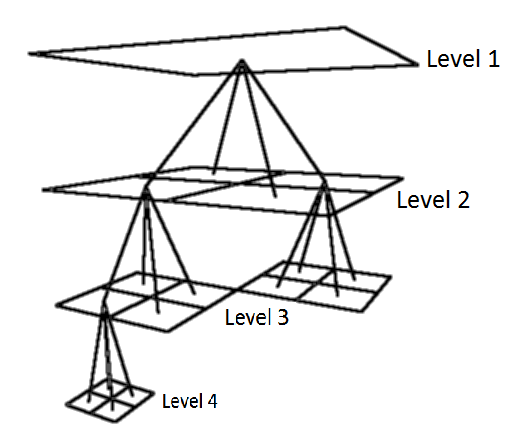
\includegraphics[width=6cm]{images/ch1/QuadTreeHierarchy}
%\caption{A visualization of the QT hierarchy}
%\label{QuadTreeHierarchy}
%\end{figure}

\subsubsection{The Octree}

The OT works similarly to the QT, however, instead of beginning with a square encompassing the entire region, a cube is used to enclose a 3D space. Similarly to the QT, an error metric is used to decide whether to split up the space or leave it unchanged. Each split operation divides each coordinate ($x,y,z$) by two, leaving 8 subspaces. Figure \ref{OctreeExample} shows this decomposition. The further each cube is split, the more the OT resembles the model being compressed. In the QT and OT, nodes which have not been split are called leaf nodes and the function which decides whether a node should be split is called the leaf criterion. 

%\begin{figure}[!h]
%\centering
%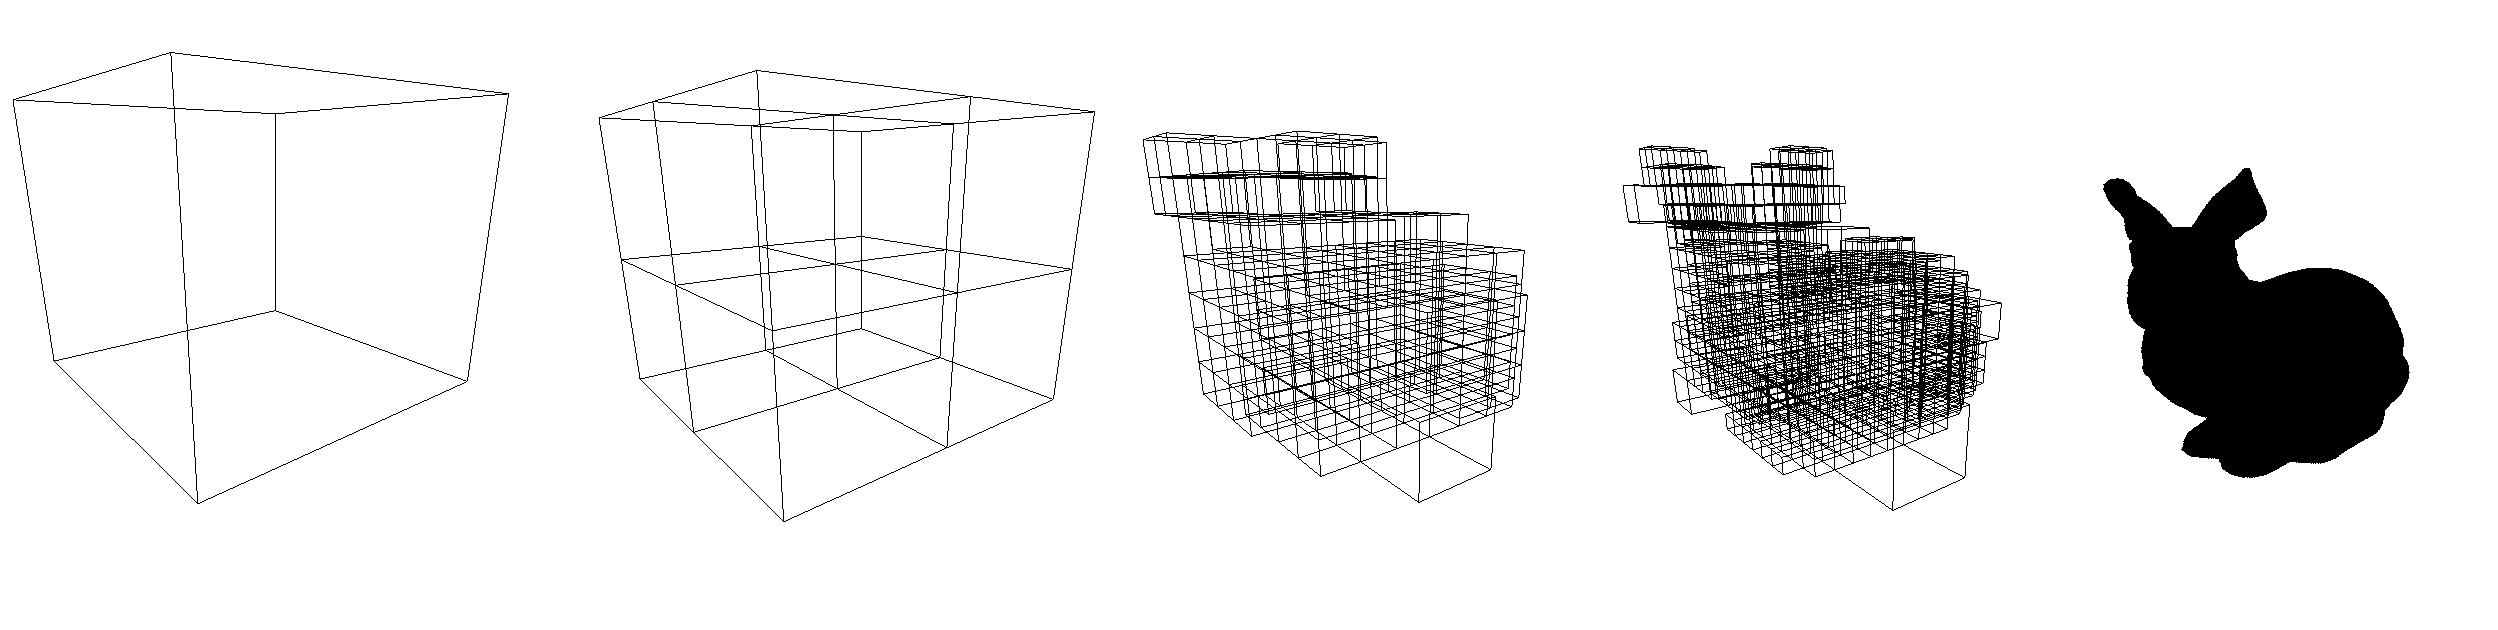
\includegraphics[width=16cm]{images/ch1/OctreeExample}
%\caption{Visualization of OT Decomposition}
%\label{OctreeExample}
%\end{figure}

\subsubsection{General Tree Storage}

The goal of the OT and the QT is to store the size and attributes of each node implicitly. There are two main methods of representation, a packed traversal of the tree and a linear tree. The packed traversal method stores the hierarchy using a pre-defined traversal of the tree, and typically follows one of two orderings. These are, breadth-first traversal and depth-first traversal, these orderings are shown in figure \ref{TreeTraversalExample}. The depth-first traversal starts at the root, then works it's way down, top to bottom, then left to right of the tree. In essence, it travels to a node's children before considering its neighbours. In contrast, the breadth-first traversal goes to all nodes which are at the same depth before continuing on to lower levels. 

%\begin{figure}[!h]
%\centering
%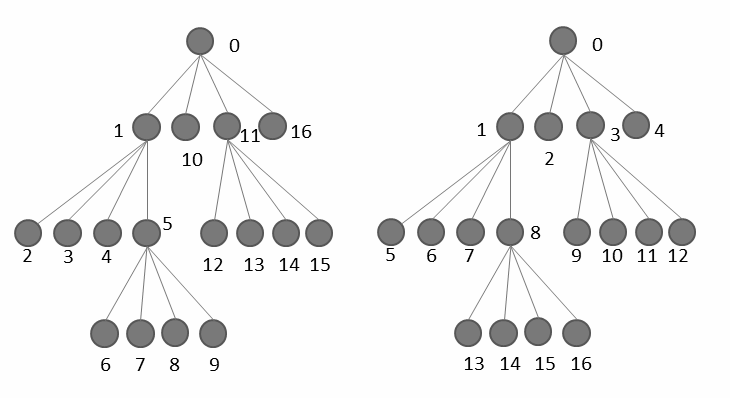
\includegraphics[width=12cm]{images/ch1/TreeTraversalExample}
%\caption{Tree Traversals, Left: Depth First Traversal, Right Breadth First Traversal}
%\label{TreeTraversalExample}
%\end{figure}

Encoding these two tree traversal methods requires one nibble (4 bits) for a QT node, and one byte (8 bits) for an OT node, where the bits represent the structure of the sub-node. For example, the QT node bit sequence, $1001_2$ means that the node has two children (corresponding to the ones), the sequence $0000_2$ means the node is a leaf node. Each bit position indexes a child node using a pre-determined ordering. An example of a possible ordering for a quadrant and an octant is shown in figure \ref{ChildOrderExample}, both breadth-first and depth-first traversals use the same index method, the difference lies only in the order which nodes are visited. 

%\begin{figure}[!h]
%\centering
%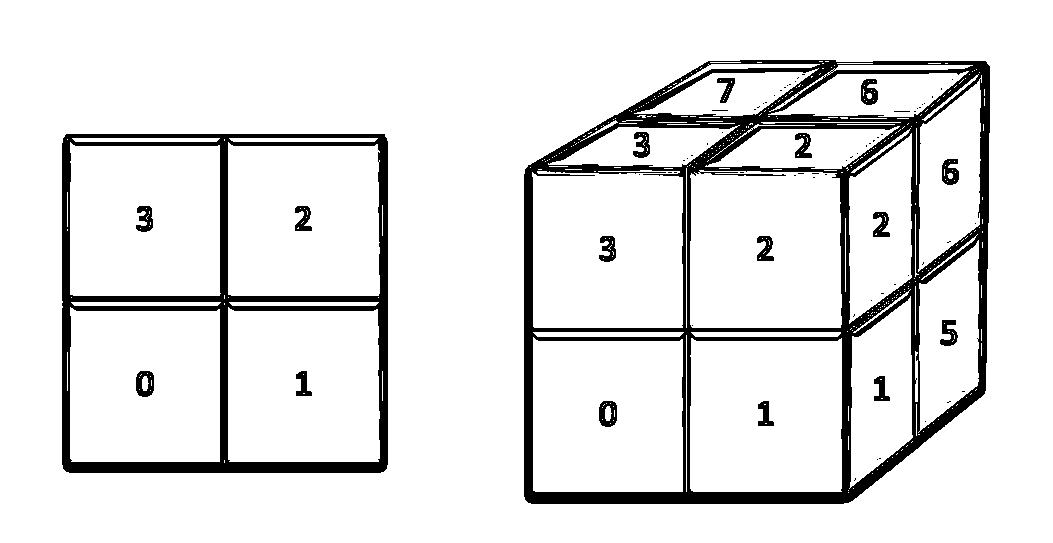
\includegraphics[width=12cm]{images/ch1/ChildOrderExample}
%\caption{A possible child ordering for the QT (left), and the OT (right).}
%\label{ChildOrderExample}
%\end{figure}

The linear tree representation stores each leaf node individually. Each leaf is encoded as the pathway from the root to the leaf itself. This method was investigated in the 1980s \cite{Gargantini82Effective,Yufei88Octcodes}, but has not been used much in modern compression algorithms due to its inefficiency compared with the packed traversal method. An example of this structure is shown in figure \ref{LinearCellCodeRepresentation}, where each node: $a$, $b$, $c$, $\dots$ , $m$  is encoded as a variable length traversal path. The QT and OT are widely used in image \cite{Varma12Application} and 3D compression \cite{Schnabel06Octree}. Hanan Samet \cite{Samet88Fund1} presents an introduction to both of these structures, he also describes both tree storage methods in depth. 

%\begin{figure}[!h]
%\centering
%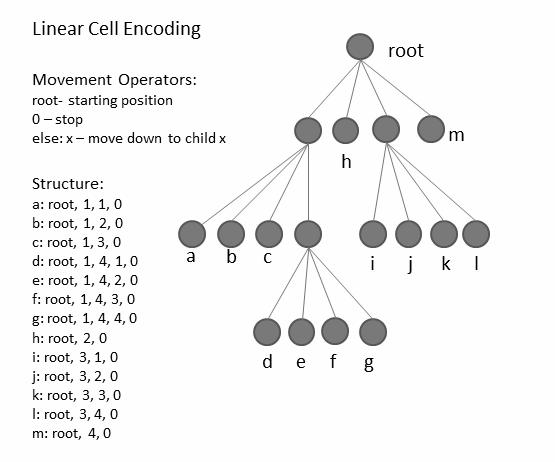
\includegraphics[width=12cm]{images/ch1/LinearCellCodeRepresentation}
%\caption{A Linear Tree Code Representation Example}
%\label{LinearCellCodeRepresentation}
%\end{figure}

\subsubsection{Other Hierarchical Structures}

Other Hierarchical structures have also been developed and researched in the context of compression. These include: the K-D tree \cite{Gandoin02Progressive}, BSP tree \cite{Radha96Image} and Wedgelets \cite{Donoho99Wedgelets,Wakin02Rate}. These structures are further explained in section 3.2 along with other QT modifications \cite{Varma12Application,Shukla05Rate,Gonzalez07ShadeTree,Kassim09Hierarchical, Lincoln13Interpolating}.

%\begin{figure}[!h]
%\centering
%\includegraphics[width=16cm]{images/ch1/DIBRExample}
%\caption{An example of a DIBR called a Layered Depth Image.}
%\label{DIBRExample}
%\end{figure}

\subsection{Depth Image Based Representations}

The Depth Image Based Representation (DIBR) has become increasingly popular in the past few years due to its ability to store photo-realistic graphics. This representation uses one or more 2D images to represent 3D objects. The most popular DIBR format was developed by Shade \textit{et al.} \cite{Shade98Layered}, and is called the Layered Depth Image (LDI). This method uses a special kind of 2D image to represent 3D objects. The image is generated using an orthographic projection of the model, where each coordinate has a variable sized list of pixels, ordered by depth. Layer is the term given to an image made up of depth values, each of which has a particular order in the coordinate list. For example, the first layer would show the closest points from the orthographic camera to the model. In order to obtain the second layer, all particles coinciding with the first layer of the object are removed, then the closest particles to the camera are used for the second layer. Figure \ref{DIBRExample} shows an example of the LDI. The figure contains the ordered layers read left to right, top to bottom. LDI data becomes more sparse at each successive layer, this is a common problem associated with the LDI approach. 

\subsection{A Comparison of Representation Schemes}

Each object representation has advantages and disadvantages categorized by: storage, transmission, processing and visualization. Table \ref{table:RepresentationComparison} presents these advantages and disadvantages. This table provides an original comparison of 3D representations. Kaufman \textit{et al.} compared the volumetric representation with the polygonal mesh \cite{Kaufman93Volume}. Since 2D data moved from vector (2D shapes) to raster (pixel arrays), Kaufman \textit{et al.} predicted 3D graphics would make a similar transition from mesh to volumetric. This has not been the case, as research and development has still paid more attention to the polygonal mesh.


\afterpage{%
\clearpage% Flush earlier floats (otherwise order might not be correct)
\thispagestyle{empty}% empty page style (?)
\begin{landscape}% Landscape page
\centering % Center table
\begin{table}
\begin{tabular}[c]{ |p{2.1cm}|p{3cm}|p{3cm}|p{3cm}|p{3cm}|p{3cm}| }
  \hline
  \multicolumn{6}{|c|}{Advantages and Disadvantages of 3D Object Representations}
  \\
  \hline
  Category & Polygonal Mesh & Volumetric & Point Cloud & Hierarchical & DBIR\\
  \hline
  Storage \& Transmission & Storage size and transmission time both dependend on object complexity.
 & Storage size is large and transmission is long but constant for a particular volume buffer size.
 & Densely sampled point clouds can take up huge amounts of storage space resulting in lengthy transmission times.
 & Storage size is small as data is automatically compressed, transmission is fast because of the progressive nature of the structure.
 & Storage Size is smaller than the Volumetric Representation, but is somewhat dependent on object complexity.
\\
\hline
  Processing
 & Processing is slow and difficult for complex objects, requiring computationally demanding computer graphics algorithms for processing.
 & Typical Signal Processing algorithms can be applied, making processing simple, but large volume buffers slow processing speed.
 & Easier to process relative to mesh data, as no connectivity must be processed. Storage Size can slow processing speed.
 & Easier to process than the Mesh representation but more difficult to process then volumetric data, various processing algorithms have been developed for this structure. 
 & Similar to the volumetric representation, some signal processing algorithms can be directly applied.
\\
  \hline
  Visualization
 & Very fast, making use of widely accessible graphics hardware processors. Is dependent on object complexity.
 & Independent of scene complexity, but suffers from aliasing. For hardware processing, custom or programmable hardware must be employed.
 & Sparse Clouds are not visually pleasing, dense can represent photo-realistic graphics but are slow to visualize.
 & Ray-Tracing based visualization algorithms are a simple search through the hierarchy, making visualization fast with relatively small storage space. Can suffer from aliasing.
 & Visualization involves specialized algorithms which can be used to speed up visualization. DBIR can represent photo-realistic scenes but using the special viewing algorithms, distortion can occur.
\\
  \hline
\end{tabular}
\caption{A table comparing different representation schemes}
\label{table:RepresentationComparison}
\end{table}
\end{landscape}
\clearpage% Flush page
}
\newpage
\section{Mesh Based Compression}

Mesh compression algorithms are divided into single-rate and progressive. Single-rate codecs encode the entire 3D object into a single data file, the decoder must have access to the entire data file before decompression can be performed. Progressive codecs can decode the model progressively. The more data sent across the communication channel, the more detail the receiver can decode and visualize. 

\subsection{Single-Rate Codecs}

\subsubsection{Introduction}

Single-rate mesh codecs are typically connectivity based methods. These methods compress connectivity information by coding vertices in a special order. During decompression, the connectivity information is re-calculated from this ordering. These methods are lossless codecs, and include: the triangle fan and strip \cite{Deering95Geometry}, the layered triangle structure \cite{Bajaj99SingleRate}, topological surgery \cite{Taubin98Geometric} and the valence driven approach \cite{touma98triangle,Alliez01Valence-Driven}. 

\subsubsection{The Triangle Fan and The Triangle Strip}

Two mesh structures often used in rendering are the triangle fan and triangle strip. The triangle fan stores triangles which share a vertex. Figure \ref{TriangleFanPicture} shows an example of a triangle fan. In the fan, a single vertex is stored ($V_0$), followed by a set of ordered vertices, $\{V_1, V_2 \cdots, V_n\}$. These form a set of triangles $\{T_0, T_1, \cdots, T_n\}$ such that, for each vertex $V_k$, $(V_{0}, V_k, V_{k+1})$ form triangle $T_{k-1}$, and $T_n$ is formed by $(V_{0}, V_{n}, V_{1})$. The code for the triangle fan in the figure consists of vertices, $\{V_0, V_1, V_2, V_3, V_4, V_5, V_6\}$. From this list, the original vertex and connectivity information can be recovered.

%\begin{figure}[!t]
%\centering
%\includegraphics[width=6cm]{images/ch1/trianglefan}
%\caption{Triangle Fan}
%\label{TriangleFanPicture}
%\end{figure}

The triangle strip stores triangles which share edges. If compressing the mesh in figure \ref{TriangleStripPicture}, the triangle strip would encode triangles in the order, ($T_0$, $T_1$, $T_2$, $T_3$, $T_4$, $T_5$, $T_6$, $T_7$, $T_8$) as these triangles share an edge with both, the previous and next triangle in the list. An example of the triangle strip algorithm is as follows, the algorithm starts with two randomly chosen connected vertices, $V_3$ and $V_0$. The next vertex which completes a triangle with these is $V_2$, this forms $T_0$. Vertices $V_0, V_3$ and $V_2$ form a set called, the current set. To store a second triangle, one vertex is removed from the current set, and a new vertex is appended. For example, to store $T_1$, vertex $V_0$ is removed from the current set and $V_6$ is added. In this fashion, the rest of the triangles are coded using the ordered vertex list, $V_0$, $V_3$, $V_2$, $V_6$, $V_7$, $V_9$, $V_8$, $V_5$, $V_3$, $V_4$ and $V_1$.

In order to decode the strip, Deering \cite{Deering95Geometry} used both a vertex and command list. Deering's version of the algorithm iterates over the vertex list, using the commands to decide which vertex in the current set must be removed. These commands include, 'O' -- replace oldest index and 'M' -- replace middle index. The construction of the vertex and command lists begins with a randomly selected triangle $T_0$ and two empty lists: $C$ (connectivity) and $G$ (geometry). The current set is formed using the vertices of $T_0$ ($V_3, V_0, V_2$) and each of these vertices are added to $G$, which becomes, $(V_3, V_0, V_2)$. Then, $T_1$ must be added to the list, so $V_6$ is added to the current set and replaces $V_0$, so the current set is updated to, ${V_3, V_2, V_6}$. Since the removed vertex $V_0$ was the middle element, $M$ is added to set C. Following this pattern, G becomes ($V_3$, $V_0$, $V_2$, $V_6$, $V_7$, $V_9$, $V_8$, $V_5$, $V_3$, $V_4$, $V_1$) and C becomes ($M$, $M$, $O$, $O$, $M$, $M$, $O$, $O$).

%\begin{figure}[!t]
%\centering
%\includegraphics[width=6cm]{images/ch1/trianglestrip}
%\caption{Triangle Strip}
%\label{TriangleStripPicture}
%\end{figure}

\subsubsection{The Generalized Triangle Strip}

The triangle strip is inefficient because the vertices in the geometry ($G$) list are repeated. Michael Deering \cite{Deering95Geometry} came up with a technique called the Generalized Triangle Strip which improves upon the triangle strip method and reduces the severity of this problem. To do this, Deering uses an extra buffer called the mesh buffer, which stores up to 16 vertices. Instead of repeating a vertex, a reference of it is appended to the mesh buffer, this reference requires less storage space. In order to generate the mesh buffer, an extra code is stored, telling the decoder to add vertices into the mesh buffer.

The generalized triangle strip works in four stages: the vertex and command list are formed, the vertex list is quantized (usually $8-16$ bits per coordinate), the quantized vertices are delta coded (the differential is stored instead of direct values, $V_k = V_k - V_{k-1}$) and finally the delta code and the command list are Huffman coded. 

The generalized triangle strip scheme stores connectivity information losslessly, however, it performs lossy compression of vertex data. Deering performed visual tests and found that quantization of vertex data to 48 bits per vertex (16 bits per coordinate) does not produce noticeable perceptual error. This assumption has been extended to many compression schemes. Deering's approach is not as efficient as most of the techniques in this survey, and it cannot encode non-manifold polygon mesh objects.

\subsubsection{Topological Surgery}

In order to handle non-manifold mesh types, Taubin \textit{et al.} \cite{Taubin98Geometric} came up with a method based on Deering's generalized triangle strip which splits a model up into sets of simple polygons. Taubin \textit{et al.} use a vertex spanning tree along with a set of jump edges to split the model into manifold sections. This is a lossless connectivity codec, which improves upon the generalized triangle strip. It works by organising vertices into a vertex spanning tree, each vertex in the tree is then predicted using 2, 3 or 4 of its ancestors, the correction vectors are then quantized and entropy coded. For connectivity, Taubin \textit{et al.} prove that if an edge is not in the vertex spanning tree, it belongs to a set they call the marching edge set. This marching edge set is used as an ordering for a triangle strip called the triangle spanning tree, which is then entropy encoded. This method is a slight improvement over Deering's approach \cite{Deering95Geometry}, however, it still stores some vertices repeatedly.

\subsubsection{Single Resolution Compression} 

Bajaj \textit{et al.} \cite{Bajaj99SingleRate} solved the vertex repetition problem with their layered triangle structure. This partitions triangles into layers which are defined by a vertex list. These layers are categorized as: contours, branching points, triangle fans, triangle strips and exceptional triangle strips. 
An example of this structure, with three layers, is shown in figure \ref{TriangleLayerPicture}. Each layer is visually coded, the light grey layer is a triangle fan and the white and dark grey layers are triangle strips. The dark grey layer contains two bubble triangles which are marked with a white circle. Bubble triangles form part of a strip's perimeter and are encoded within the strip for efficiency purposes. Strips with bubble triangles are called exceptional triangle strips. A vertex which connects two layers is called a branching point.

Aside from the vertex list, this structure must encode: the number of layers, the layout of each layer, as well as the fans and strips making up each layer. Vertices are delta coded, quantized and entropy encoded. For each vertex, spherical coordinate errors are encoded instead of vector errors, and each coordinate is quantized differently. Bajaj \textit{et al.} use a static Huffman coder for their triangle strip representation, which they claim increases connectivity compression by around $25\%$. This is based on the fact that the command list most often oscillates like a digital clock signal (eg. $O$, $M$, $O$, $M$, $\dots$, $O$, $M$).

%\begin{figure}[!h]
%\centering
%\includegraphics[width=6cm]{images/ch1/TriangleLayer}
%\caption{Layered Triangle Strip}
%\label{TriangleLayerPicture}
%\end{figure}

In order to summarize the research presented so far, table \ref{table:schemeComparisonTable1} is used to compare the previously discussed methods. Results are compared when input models have similar vertex and triangle counts. The results show that the Layered Triangle structure by Bajaj \textit{et al.} \cite{Bajaj99SingleRate} has the best performance and that the method by Taubin \textit{et al.} \cite{Taubin98Geometric} outperforms Deering's \cite{Deering95Geometry} generalized triangle strip.

\begin{table}[!t]
\begin{tabular}[c]{|l|l|l|l|l|l|}
\hline
\multicolumn{6}{|c|}{Codec Comparison Table}\\
\hline
Scheme & Object Name & No. Vertices & No. Triangles & No. Bytes & bits per vertex\\
\hline
Deering & triceratops & 3020 & 6039 & 46237 & 122.4821192\\
Taubin \textit{et al.} & bunny-26 & 3466 & 6816 & 6968 & 16.083\\
Taubin \textit{et al.} & bunny-11 & 6728 & 13232 & 14555 & 17.307\\
Bajaj \textit{et al.} & Honda & 6797 & 13594 & 3688 & 4.341\\
Deering & 57Chevy & 15881 & 31762 & 141830 & 71.446\\
Taubin \textit{et al.} & Crocodile & 18242 & 36064 & 80056 & 35.108\\
Bajaj \textit{et al.} & Crocodile & 17202 & 34404 & 9523 & 4.429\\
\hline
\end{tabular}
\caption{A table comparing strip based compression schemes \cite{Deering95Geometry,Taubin98Geometric} and the layered triangle structure \cite{Bajaj99SingleRate}.}
\label{table:schemeComparisonTable1}
\end{table}

\subsubsection{Triangle Mesh Compression}

Valence based methods are more efficient than the triangle strip based approaches. The earliest method was published by Touma and Gotsman \cite{touma98triangle} in their paper entitled Triangle Mesh Compression. This method compresses orientable triangle meshes and is a connectivity based codec. Vertex data is uniformly quantized and entropy coded. The connectivity compression system is based on the observation that connected vertices may be ordered in a counter-clockwise and consistent manner if the mesh is orientable and manifold. 

The method begins with an arbitrarily chosen triangle, and a chosen focus vertex from the triangle. Beginning with the three vertices in the triangle and extending to vertices incident to the focus, a counter-clockwise walk of these vertices is performed, and the degree of each vertex is stored in the same linear order using an add command. When the degree of each vertex connected to the focus is stored, the next vertex in the counter-clockwise order becomes the new focus. If this list intersects itself, it is split in half, using a split command. The split operation is required only when the input mesh has more than one genus (the genus of a mesh is the number of handles added to the section of the mesh which is manifold). Once two split lists are processed, the two partitions are merged using a merge command. This procedure ends when all edges are traversed.

Touma and Gotsman have stated that their structure requires mostly add commands with some split commands and few merge commands and that the average degree for vertices is 6. Huffman and run-length coding are performed on the connectivity data, which results in a coding rate of 1 bpv for standard input and 0.2 bpv for meshes of regular connectivity (where most vertices share a common degree). This method is often cited as one of the state of the art single-rate connectivity codecs. The main problem with this codec is its ability to efficiently compress irregular mesh data. 

\subsubsection{Valence Driven Connectivity Coding}

Touma and Gotsman's method suffered when topology was not regular. Alliez \& Desbrun \cite{Alliez01Valence-Driven} came up with a solution which improves its ability to compress irregular topological mesh information, they call this method the valence driven approach. For irregular mesh data, this codec improves Touma and Gotsman's compression ratio by 15\%. In their paper Alliez \& Desbrun also provide theoretical bounds for their codec. To improve the method by Touma and Gotsman, they set out to reduce the number of split codes when walking through the mesh. This is accomplished by selectively choosing the next focus vertex to be the one with the minimum number of processed neighbours. This reduces the number of split and merge commands required. Then they use an arithmetic coder instead of Huffman coding.

To compare the two valence driven approaches, table \ref{table:schemeComparisonTable2} summarizes results from Alliez \& Desbrun \cite{Alliez01Valence-Driven} and Touma \& Gotsman \cite{touma98triangle}. Alliez \& Desbrun's approach outperforms Touma \& Gotsman's on different input data in terms of bit rate. Michael Deering's approach was added to show the performance of the valence driven approach relative to a strip based method.
\begin{table}[!h]
\begin{tabular}[c]{|l|l|l|l|l|l|}
\hline
\multicolumn{6}{|c|}{Codec Comparison Table 2}\\
\hline
Scheme & Object Name & No. Vertices & No. Triangles & No. Bytes & bpv\\
\hline
Deering & triceratops & 3020 & 6039 & 46237 & 122.5\\
Touma \& Gotsman & triceratops & 2832 & 5660 & 778.8 & 2.2\\
Alliez \& Desbrun & triceratops & 2832 & 5660 & 665.52 & 1.88\\
Touma \& Gotsman & bunny & 15000 & 29783 & 3870 & 2.064\\
Alliez \& Desbrun & bunny & 15000 & 29783 & 3713 & 1.98\\
Touma \& Gotsman & fandisk & 6475 & 12946 & 874 & 1.08\\
Alliez \& Desbrun & fandisk & 6475 & 12946 & 826 & 1.02\\
\hline
\end{tabular}
\caption{A table comparing valence based compression schemes \cite{Alliez01Valence-Driven,touma98triangle}}
\label{table:schemeComparisonTable2}
\end{table}
\subsection{Progressive Codecs}

\subsubsection{Introduction}

Current research focusses on progressive compression due to its transmission advantage. Most progressive schemes perform simplification operations on a 3D object, transforming it into a coarse mesh called the base mesh. Each simplification operation can be reversed if the details of it are known. These simplification operations are sent across a communication channel with the base mesh. At the receiver end, the original model is decoded using the base mesh and the reverse simplification operations. Some progressive codecs do not use simplification operations, these include: hierarchical, wavelet and transform based codecs. 

\subsubsection{Progressive Meshes}

Hugues Hoppe \cite{Hoppe96Progressive} first used simplification to create a progressive compression scheme for 3D models. This codec is a multi-resolution lossless codec, which provides smooth transitions between simplification levels. Hoppe states that for any 3D model termed $M_N$, $N$ simplification operations can be used to simplify the original model into a set of meshes $\{M_N , M_{N-1} , \cdots , M_2 , M_1, M_0 \}$ called levels of detail, where $M_0$ is the base mesh. 

Hoppe uses a simplification operation called the edge collapse. It first chooses an edge, then converts its two vertices into a single vertex defined at the center of the edge. Any triangles and edges incident to the original vertices are then connected to this new vertex. This operation can be reversed by splitting this new vertex, but only if the affected triangles and original connectivity are known. The reverse operation of the edge collapse is called the vertex split.

Hoppe uses the generalized triangle strip to compress the coarse mesh. Correction vectors are used to predict the original vertices, these are quantized to 16 bits and Huffman coded.  A slow but optimal appearance preserving metric is used to decide the order which edges are collapsed. Hoppe also devised a process called geomorphing, which takes each vertex split operation and slows it down by interpolating the two vertices slowly back to their original positions. The geomorphing procedure ensures smooth transitions between each level of detail. 

\subsubsection{Colour Coded Triangle Mesh Compression}

In their progressive and lossless mesh codec, Cohen-Or, Levin \& Remez \cite{CohenOr99Progressive} use an alternative simplification operation called the vertex removal. This operation chooses vertices to remove from the original mesh. After one of these operations, a re-triangulation procedure is required to close the gap left behind. The triangles involved in this operation are uniformly referred to as a patch. The vertex removal operation is stored using a correction vector to predict the location of the original vertex, the center of the patch is used as this predictor. Each triangle in a patch is categorized by a colour code and triangles sharing an edge must have different codes. These codes are used to decode the original connectivity information between the removed vertex and the vertices in the patch. The colour codes are further compressed using LZ compression. This codec is proven to outperform Hoppe's \cite{Hoppe96Progressive} progressive mesh codec.

\subsubsection{Low Valence Based Simplification}

Alliez \& Desbrun \cite{Alliez01Progressive} developed another valence based codec, this one has progressive properties. It is based on the vertex removal operation and is a lossless codec. This method is suited to densely sampled mesh data. When analysing the vertex removal operation, Alliez \& Desbrun made an observation, when a vertex is removed and the hole is re-triangulated, the valences of the remaining vertices depend on the valence of the removed vertex. If the removed vertex had a valence above six then the valences of the remaining vertices increases. This increases entropy and creates more distortion than removing a vertex with a low valence. Using this observation, their scheme selects vertices with low valences to be removed first.

Each triangle can be part of at most one patch, and patches are defined relative to a previous patch. Each simplification operation is reversed using the: correction vectors, patch valences and original connectivity information. Before transmission, this data is arithmetic coded. Alliez \& Desbrun state their algorithm compresses arbitrary meshes at around $3.7$ bpv, which improves upon the compression of Cohen-Or, Levin \& Remez \cite{CohenOr99Progressive} by around $40\%$.

\subsubsection{Embedded Mesh Codec}

Li \& Kuo \cite{Li98Progressive} developed a progressive codec called the embedded mesh codec, it is based on the vertex removal operation. They call their technique embedded because it embeds the coarse mesh along with the fine details required to restore it to its original state. The vertex bit stream and the simplification operations are multiplexed using two thresholds as selectors, this maximizes rate-distortion performance. The vertex data is stored using a local prediction technique, and the multiplexing is performed layer by layer. Li \& Kuo use the distance from a vertex to the average of its neighbourhood as a metric in order to select which vertex to remove next, each vertex removal operation is encoded using a look-up table. This method outperforms Hoppe's \cite{Hoppe96Progressive} in terms of bit rate.

\subsubsection{Spectral Codecs}

Karni \& Gotsman \cite{Karni00Spectral} designed a progressive, geometry-driven mesh codec based on spectral compression. They point out that most codecs are advertised as lossless, but are actually lossy, because they perform quantization on the vertex data. This lead Karni \& Gotsman to devise a lossy coding scheme similar to JPEG image compression. 

The scheme first computes a set of basis functions for the model. This process involves computing the eigenvectors of an $n\times n$ sparse matrix. Due to this requirement, if $n$ is too large, numerical break-down (compounding round-off errors when solving a system of equations) can occur. Therefore they generalization that, a mesh with over $1000$ vertices is impractical to process. To handle large mesh inputs, Karni \& Gotsman use a mesh partitioning algorithm to break up the mesh, where each sub-mesh (partition) is compressed separately. Once the basis functions are calculated, the coefficients are quantized, then the list of coefficients are truncated and entropy coded. Quantization is typically performed at 10 to 16 bits per coordinate. The amount of coefficients chosen (during truncation) to represent the mesh adversely affects the rate-distortion. 

This scheme by Karni \& Gotsman outperforms the valence based method of Touma \& Gotsman \cite{touma98triangle} at coarse quantization levels. Results show that for a much smaller file size, the spectral scheme can encode a smoother and higher quality mesh compared with the valence based method. This comparison can be seen in figure \ref{KarniAndGotsmanVSToumaAndGotsman}, it shows that for an identical bit rate, the spectral coded model is of higher calibre.

%\begin{figure}[!h]
%\centering
%\includegraphics[width=12cm]{images/ch1/KarniAndGotsmanVSToumaAndGotsman}
%\caption{Left: The spectral coding \cite{Karni00Spectral} of the bunny at 4.1 bpv. Right: The valence based method coding of the bunny \cite{touma98triangle} at 4.1 bpv.}
%\label{KarniAndGotsmanVSToumaAndGotsman}
%\end{figure}



\subsubsection{Wavelet Based Codec}

Khodakovsky \textit{et al.} \cite{Khodakovsky00Progressive} developed a wavelet based compression scheme which performs well on densely sampled mesh models. They use their own definitions of: geometry, parameter and connectivity information to describe their methodology. Geometry is the overall shape of the model, parameter is the type of sampling used on the model and their definition of connectivity information is the same as previously described. They show that the connectivity and parameter information make the largest contribution to storage size.

In order to lower redundancy in the connectivity and parameter information, their method first performs a semi-regular sampling of model. This data is then decorrelated using the wavelet transform. The wavelet coefficients are stored in a hierarchical structure called a zerotree, this structure increases the performance of wavelet based image codecs. The basis functions of the wavelet transform are vectors in 3-space, these functions are scalar quantized (per component quantization) which requires three independent zerotree coders. The output bit streams of these coders are then multiplexed to create the final data structure. 

According to Khodakovsky \textit{et al.} arithmetic coding can be used to further compress the zerotree. Their method is shown to outperform Touma and Gotsman's in terms of rate-distortion. This scheme is useful for applications where a particular sampling of the model is unimportant.

\subsubsection{Geometry Image Representation}

Gu \textit{et al.} \cite{Gu02Geometry} designed a structure which converts any manifold mesh into a completely regular structure called a Geometry Image (GI). The GI is an rgb image created from a parametric sampling of the mesh. To generate the GI, the mesh is cut along a network of edge paths which open the mesh into a topological disk, then vertices are sampled into a 2D grid (the GI) where each point on the grid has an rgb value representing the corresponding point in 3D space. The GI has applications in both visualization and compression. Because the GI is an image, state of the art image compression algorithms can be used to compress this structure. Gu \textit{et al.} use a wavelet based image codec to compress the GI, and compare the results with the wavelet model codec by Khodakovsky \textit{et al.} \cite{Khodakovsky00Progressive}. The results show that the GI codec has slightly lower performance compared with the wavelet model codec. The GI has an advantage in that it is simple to process, however, the method used by Khodakovsky \textit{et al.} has better RD performance and is not limited to manifold models.


\subsubsection{Recent Codecs}

The following section discusses more recent codecs. Although results suggest these codecs achieve state of the art performance, they have not been widely cited as such. Peng \textit{et al.} \cite{Peng10Feature} developed a saliency based mesh codec called the Feature-oriented geometric progressive lossless mesh coder (FOLProM). Their codec can encode mesh data of arbitrary geometry and topology and is optimized to provide more bits for the salient features of the mesh, especially at low bit rates. Bayazit \textit{et al.} \cite{Bayazit103DMesh} developed another codec based on compression in the spectral domain. This codec is progressive and is based on the region adaptive transform within the spectral domain. Mamou \textit{et al.} \cite{Mamou11Multi} developed a progressive 3D mesh coding scheme based on the shape approximation prediction strategy, they call this method Shape Approximation Compression (SAC). 

\section{Depth Image Based Representation Codecs}

The DIBR uses 2D images to store 3D information. These methods are more obscure in the literature compared with mesh based research. The Layered Depth Image (LDI) is the most popular of these methods due to its ability to efficiently store and render realistic graphics.

\subsection{Layered Depth Image Techniques}

\subsubsection{Early Work}

Shade \textit{et al.} \cite{Shade98Layered} presented the first of the Depth Image Base Representation schemes. The method they presented was the LDI (see section 2.2.6). Work by Shade \textit{et al.} was focussed on visualization algorithms for the LDI but they did do some preliminary work on its compression.

\subsubsection{The Panoramic Image Map Representation}

Tsai \textit{et al.} \cite{Ming02Compression} developed a similar technique to the LDI called a PanoMap. This technique works by projecting the 3D model onto a sphere or cylinder, which is then rolled out flat, forming an image. Image compression methods are then applied to reduce storage requirements. This method suffers from a problem in that concave sections of objects are missed by the projector. When the decoder decodes a structure like this, there are large holes in the model. Tsai \textit{et al.} suggested appending missing points to the compressed structure to overcome this problem. This method is not as efficient as the LDI structure in terms of bit rate, and should be only used for non-concave models.

\subsubsection{Image Based LDI Compression}

Duan \textit{et al.} \cite{Duan03Compression} developed a compression scheme for the LDI based on image compression techniques. Because the LDI can have multiple layers per pixel, image compression cannot be directly applied. Furthermore, if multiple images are used to represent each layer, the information in the first few layers is dense, which is good, but the information in the rest of the layers is sparse. This is a problem because these images are difficult to compress. To alleviate this problem, Duan \textit{et al.} developed a scheme to compact the sparse layers before further compression is applied. Their compressed LDI is made of the following components: 3 colour channels (8 bits each), an alpha channel (8 bits), a depth value (20 bits), and a structure called a splat table which is used for efficient visualization.

Duan \textit{et al.} store the number of depth values for each coordinate in a grid which they call the Number of Layers (NOL) image. This is required by the decoder and is losslessly encoded using JPEG-LS. Each layer is then stored as an image which is compressed using a lossy wavelet image codec.

In order to compact the information in the sparse layers, a horizontal shift operation is used as a preprocessing step. This operation shifts all the non-empty pixels to the left as far as possible without overlap. Figure \ref{SparseImageCompating} illustrates the effect of this operation \cite{Duan03Compression}. This process is easily reversed using the NOL image. This compression scheme is more efficient than the PanoMap and can encode concave surfaces without loss of detail.

%\begin{figure}[!h]
%\centering
%\includegraphics[width=12cm]{images/ch1/SparseImageCompating}
%\caption{Example Image \cite{Duan03Compression} illustrating Duan \textit{et al.} method of compacting sparse image data}
%\label{SparseImageCompating}
%\end{figure}

\subsubsection{Partial Surface Based Compression}

The state of the art DIBR codec is based on surface correlation and was proposed by Park \& Kim \cite{Park10Efficient}. This codec extracts surfaces from the layers of an LDI and represents them using bezier functions. These data are then shape-adaptive DCT transformed, quantized and entropy encoded. In order to compute the surfaces, connectivity information must be generated and coded along with the representation. This method is shown to outperform other DIBR codecs as well as the original technique by Shade \textit{et al.}  \cite{Shade98Layered}.

\section{Hierarchical Codecs}

This section presents the hierarchical techniques employed in 3D model compression. These techniques all use standard OT decomposition to compress geometry data, with the exception of the K-D tree codec.

\subsection{Mesh Codecs}

\subsubsection{K-D Tree Progressive Codec}

Gandoin \& Devillers \cite{Gandoin02Progressive} designed a progressive, lossless and vertex-driven mesh codec  which uses a K-D tree to store vertex data. The K-D tree splits leaf nodes in half, this split can be along either the x, y or z axis. To compress the vertex data, the number of vertices within each node is arithmetic coded and stored along within the packed traversal of the K-D tree. This scheme compresses edges not triangles, therefore the decoder must re-calculate the triangle data based on the received edge and vertex information. This requires extra computation but the original triangle information can be restored. This codec uses the edge collapse operation for progressive compression. Prediction and arithmetic coding are then used to compress these data. Gandoin \& Devillers' algorithm can also be applied to volumetric meshes. This codec outperforms the methods by Alliez \& Desbrun \cite{Alliez01Progressive} and Cohen-Or \textit{et al.} \cite{CohenOr99Progressive} in terms of bit rate.

\subsubsection{Geometry-Guided Progressive Octree Codec}

Peng \& Kuo \cite{Peng05Progressive, Peng05Geometry-Guided} use the OT in their progressive and lossless mesh codec. This algorithm can encode a mesh of arbitrary topology, but only encodes vertex and edge information, requiring the decoder to re-calculate triangles. To achieve progressive compression, the OT is encoded using a breadth-first, packed traversal of the tree. At each level, this scheme selects the order in which nodes are sent, as this optimizes RD performance. For each refinement of the OT, a vertex split operation is also sent.

Peng \& Kuo use an 8 bit code to represent each sub-node's structure. These codes are ordered by probability and stored in a look-up table. Each 8 bit code is arithmetic coded using its tree depth and the amount of vertices within the node. Each vertex split operation is also arithmetic coded. During transmission, a node is given higher priority if it: contains many vertices, is too large or is highly isolated. Their method improves upon the K-D tree based codec of Gandoin \& Devillers \cite{Gandoin02Progressive} and has been cited as being one of the state of the art progressive mesh codecs \cite{Berjon13Objective}.

\subsubsection{The Post-Forecast Octree Codec}

Cai \& Yu \cite{Cai09Post} use an OT to encode geometric data. Their codec can also compress attribute information (normals, texture coordinates). To provide progressive transmission, they transmit a breadth-first packed traversal of the OT to the receiver. Cai \& Yu found that a fine representation of the vertices using an OT requires encoding many nodes with a single child. Rather than encoding all nodes using 8 bits (one per child), Cai \& Yu use an extra decision bit which switches between the 8 bit code, and a 3 bit code capable of representing a single child's location. Their algorithm is not as efficient as Peng \& Kuo's \cite{Peng05Geometry-Guided} and only compresses geometric data.

\subsection{Surface Codecs}

\subsubsection{A Single-Rate Volumetric \& Surface Dual Codec}

Siddiqui \textit{et al.} \cite{Siddiqui07Octree} developed a single-rate, lossless OT codec designed to encode both densely sampled mesh surfaces and volumetric data. They use OT decomposition with a rate-distortion based leaf node criterion. Decomposition is not stopped until each node contains at most, one vertex. The tree is stored using the packed traversal method. Siddiqui \textit{et al.} apply run-length coding then Huffman compression to their data structure. This scheme can encode a detailed Stanford bunny at a bit rate of 11.2 bpv. This is a higher bit rate compared with the OT codec by Peng \& Kuo \cite{Peng05Progressive, Peng05Geometry-Guided} which has the added advantage of being progressive.

\subsubsection{The Progressive Octree Particle Method}

Yemez \& Schmitt \cite{Yemez03Multilevel} use an OT to compress densely sampled point cloud data. This scheme does not preserve topology information, but is lossless in the sense that no surface detail is lost. To save storage space, a surface thinning method is applied to the OT before progressive transmission, this procedure performs checks to remove any redundant leaf nodes. The tree is transmitted in breadth-first order using the packed traversal method. This codec does not use any entropy coding and generally compresses data at 5-9 bits per triangle or 10-18 bits per vertex. Yemez \& Schmitt use a variation of the marching cubes algorithm to generate triangles from $2\times 2\times 2$ volumes. This method can also be adapted to store other attribute information.

\subsubsection{Prediction Based Octree Point Cloud Compression}

Schnabel \& Klein \cite{Schnabel06Otree-based} developed a progressive compression scheme for the point cloud representation. This method is based on the OT and uses a novel prediction scheme to predict the configuration of all nodes at a particular level. Each point is first quantized to 16 bits per coordinate and stored in the OT, which is then transmitted in a top-down, breadth-first order using the packed traversal method. At each level in the tree, a least squares approximation of the surface is used to predict the OT configuration of the next level. The order which nodes are sent is optimized per level, this improves rate-distortion performance. This method also supports the coding of attribute information by assuming it can be efficiently stored in each node.

\subsection{Depth Image Based Representation Codecs}

\subsubsection{The Octree-Image Codec}

Levkovich-Maslyuk \textit{et al.} \cite{Levkovich04Depth} devised a codec for the DIBR called the Octree-Image. The Octree-Image stores geometry data in an OT. The colours of each leaf node are stored using multiple images, which are obtained from different views. Another structure is used as a link between the OT and these colour images. To compress the Octree-Image, Levkovich-Maslyuk \textit{et al.} use the parent's substructure as the context of an adaptive arithmetic coder. The Octree-Image can represent photo-realistic images better than the mesh representation, but this codec only halves the uncompressed file size.  


\section{Conclusion}

There are many representation and compression schemes for 3D data, and the best choice of representation and codec depends application requirements. Most of the recent 3D model compression schemes have focussed on wavelet, spectral or other transform methods, with few taking advantage of recently proposed hierarchical techniques found in image compression research. The next chapter presents the SOT and describes how it makes use of such techniques.

